\chapter{Circuiti RC e RL (C3)}

Oggetto di studio di questa esperienza è l'andamento della differenza di potenziale ai capi di resistenza e capacità o induttanza.
A tal fine costruiamo un circuito con i seguenti elementi:
[disegno]

\begin{itemize}
  \item Generatore di onde
  \item Un condensatore di capacità 367 nF più errore
  \item Un'induttore di induttanza sconosciuta
  \item Un oscilloscopio con due sonde
  \item Una resistenza di 667 Ohm (più errore)
\end{itemize}

\section{Corrente impulsata}
\subsection{Procedimento}


Per simulare l'apertura e la chiusura del circuito impostiamo nel generatore la modalità onda quadra. Una sonda posta prima del condensatore mostra sullo schermo dell'oscilloscopio il segnale.  
Una seconda sonda, posta ai capi della resistenza, visualizza la forma dell'onda caratteristica della carica o della scarica di un condensatore.

Raccogliamo i dati (differenza di potenziale e tempo) dall'onda visualizzata sul display dell'oscilloscopio, tramite i cursori. Interpoliamo i dati per stimare il tempo caratteristico $\tau$ del circuito.

\subsection{Dati}

\subsubsection{Circuito RC}

Per il circuito  RC in carica, con un'onda quadra a 50 Hz come sorgente, abbiamo raccolto questi dati:
\begin{center}
\begin{tabular}{*{2}{c}}
Tempo ($\mu s$) & Ddp ($V$) \\
\midrule
0 & 18.20 \\
100 & 12.80 \\
200 & 9.00 \\
300 & 5.80 \\
400 & 4.40 \\
500 & 3.20 \\
600 & 2.20 \\
700 & 1.80 \\
800 & 1.20 \\
900 & 1.00 \\
\end{tabular}
\end{center}

Graficati:

\begin{center}
 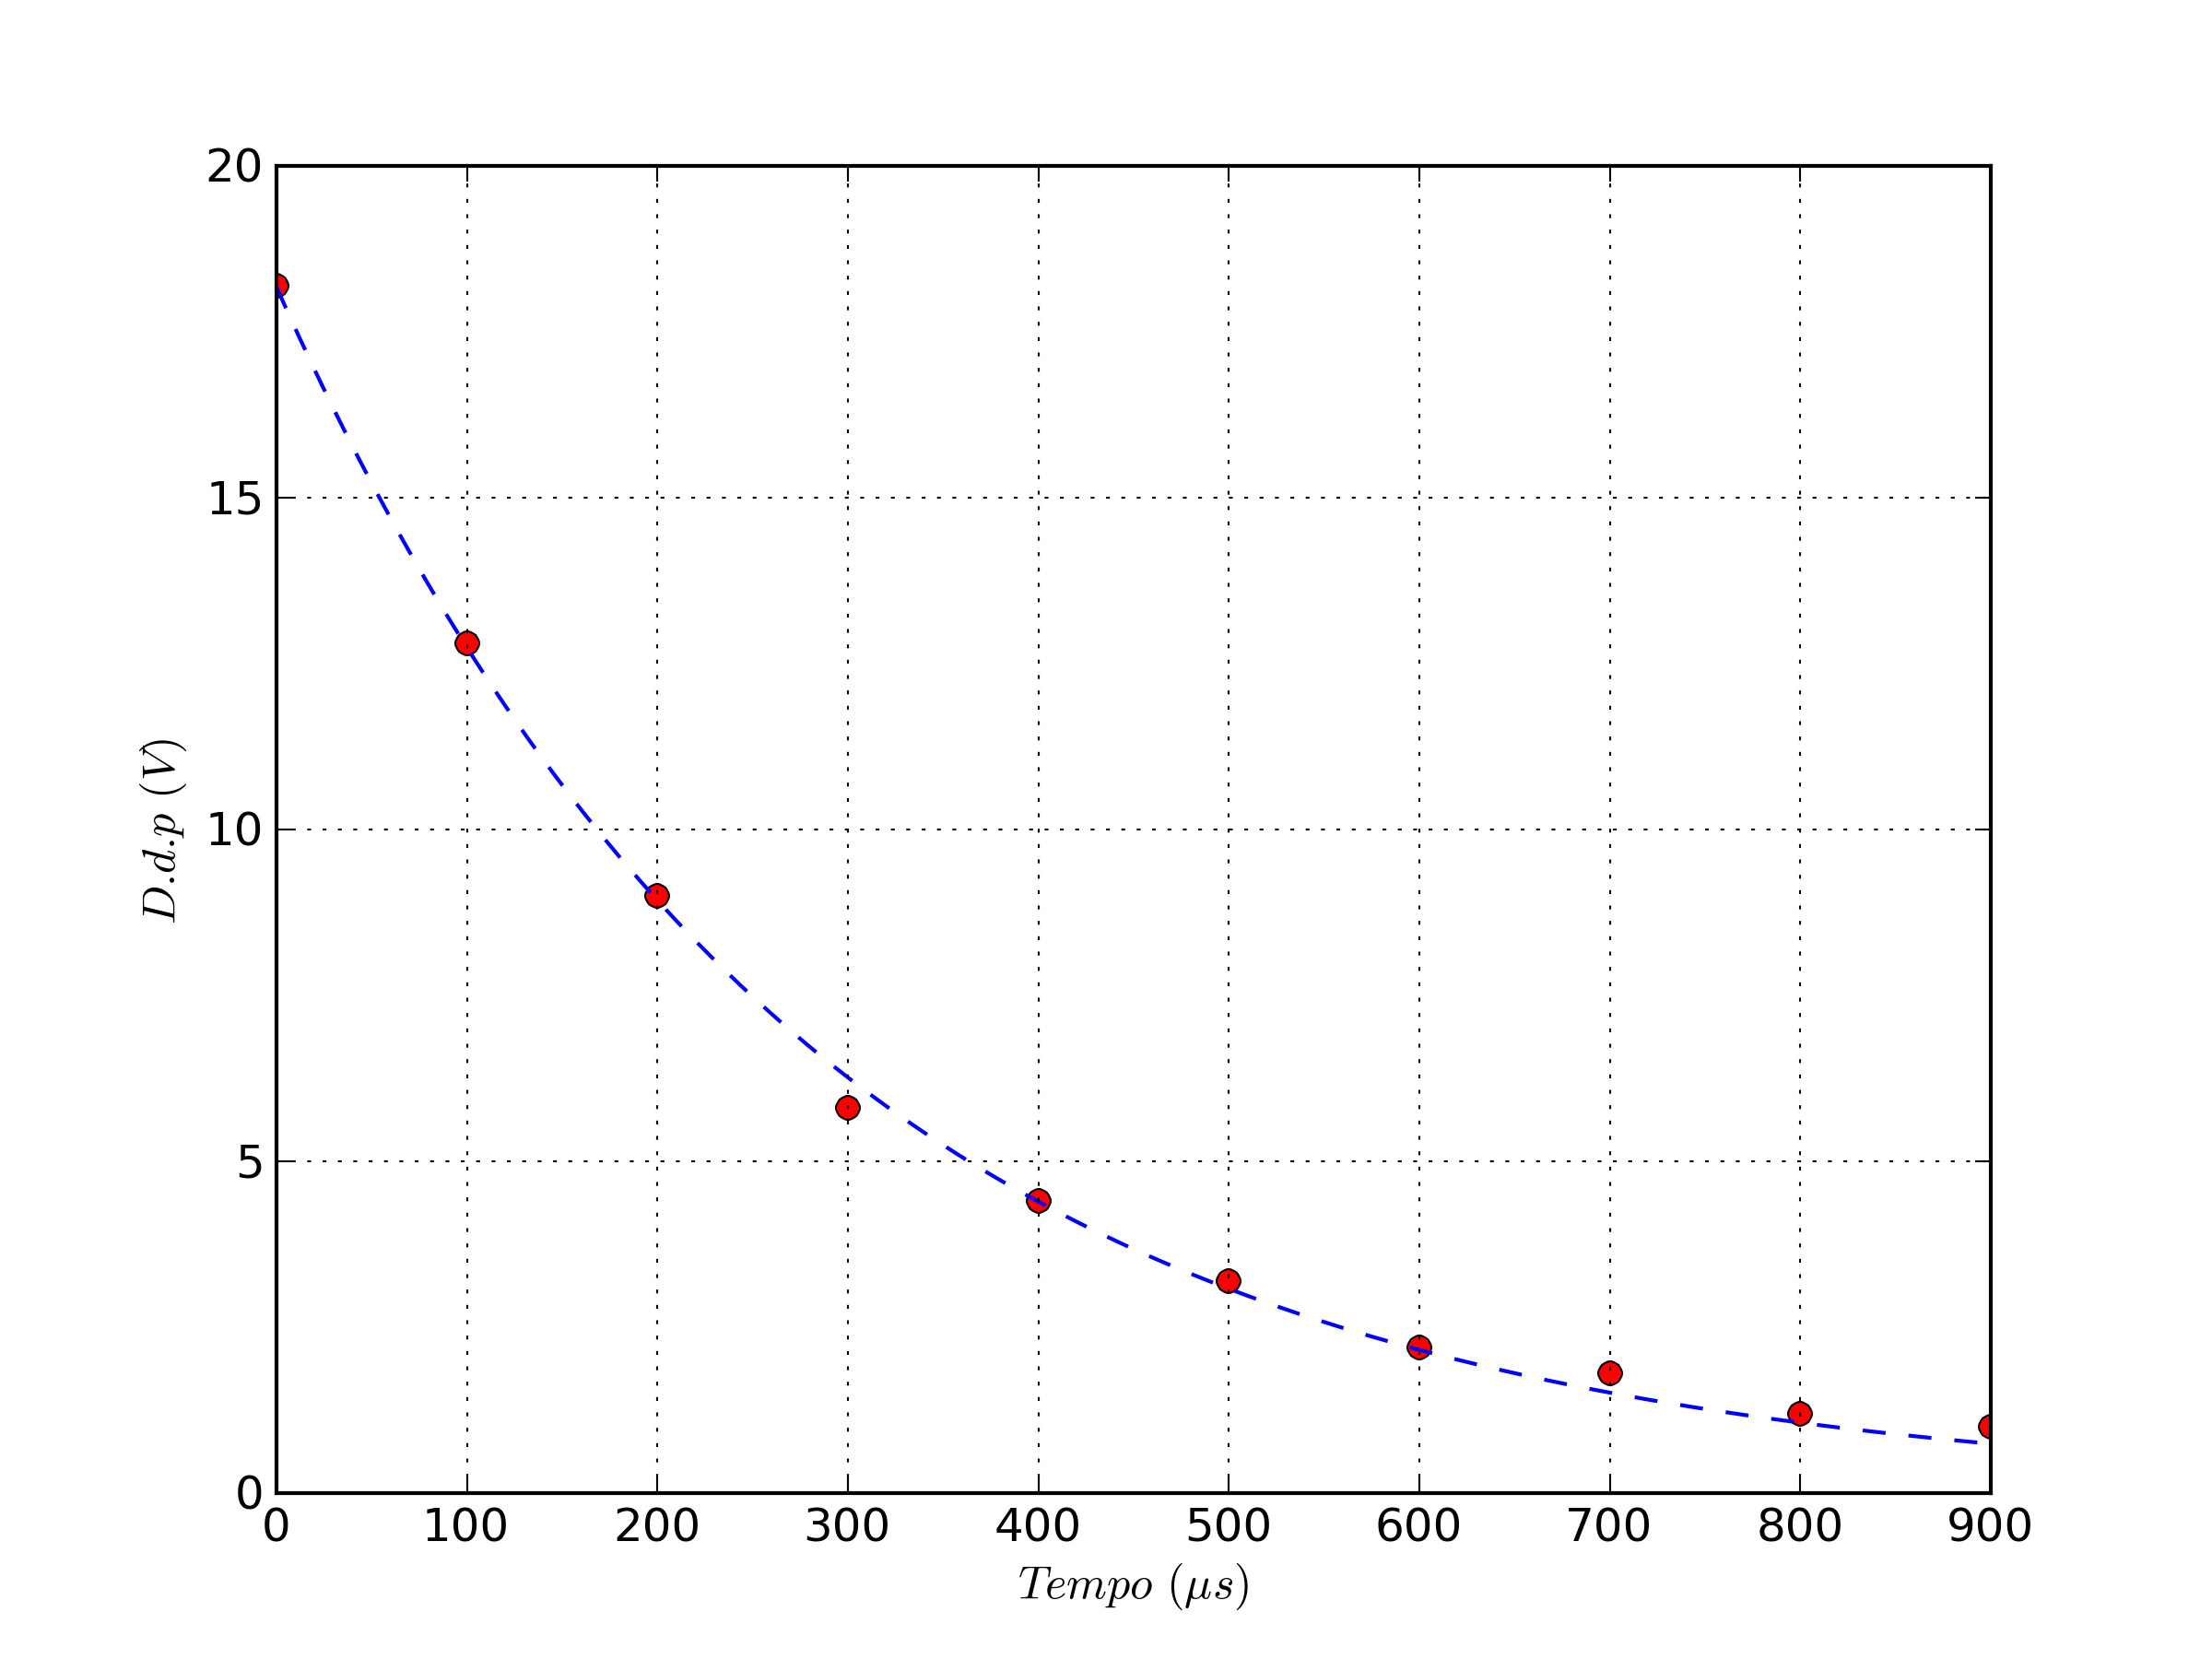
\includegraphics[scale=0.70]{grafici/C3/fitcond.png}
\end{center}



\subsubsection{Circuito RL}
Con un'onda quadra a 250 Hz, abbiamo raccolto questi dati:

\begin{center}
\begin{tabular}{*{2}{c}}
Tempo ($\mu s$) & Ddp ($V$) \\
\midrule
5 & 5.00 \\
10 & 8.00 \\
15 & 10.60 \\
20 & 12.40 \\
25 & 13.60 \\
30 & 14.60 \\
35 & 15.40 \\
40 & 16.20 \\
45 & 16.40 \\
\end{tabular}
\end{center}

Graficati:

\begin{center}
 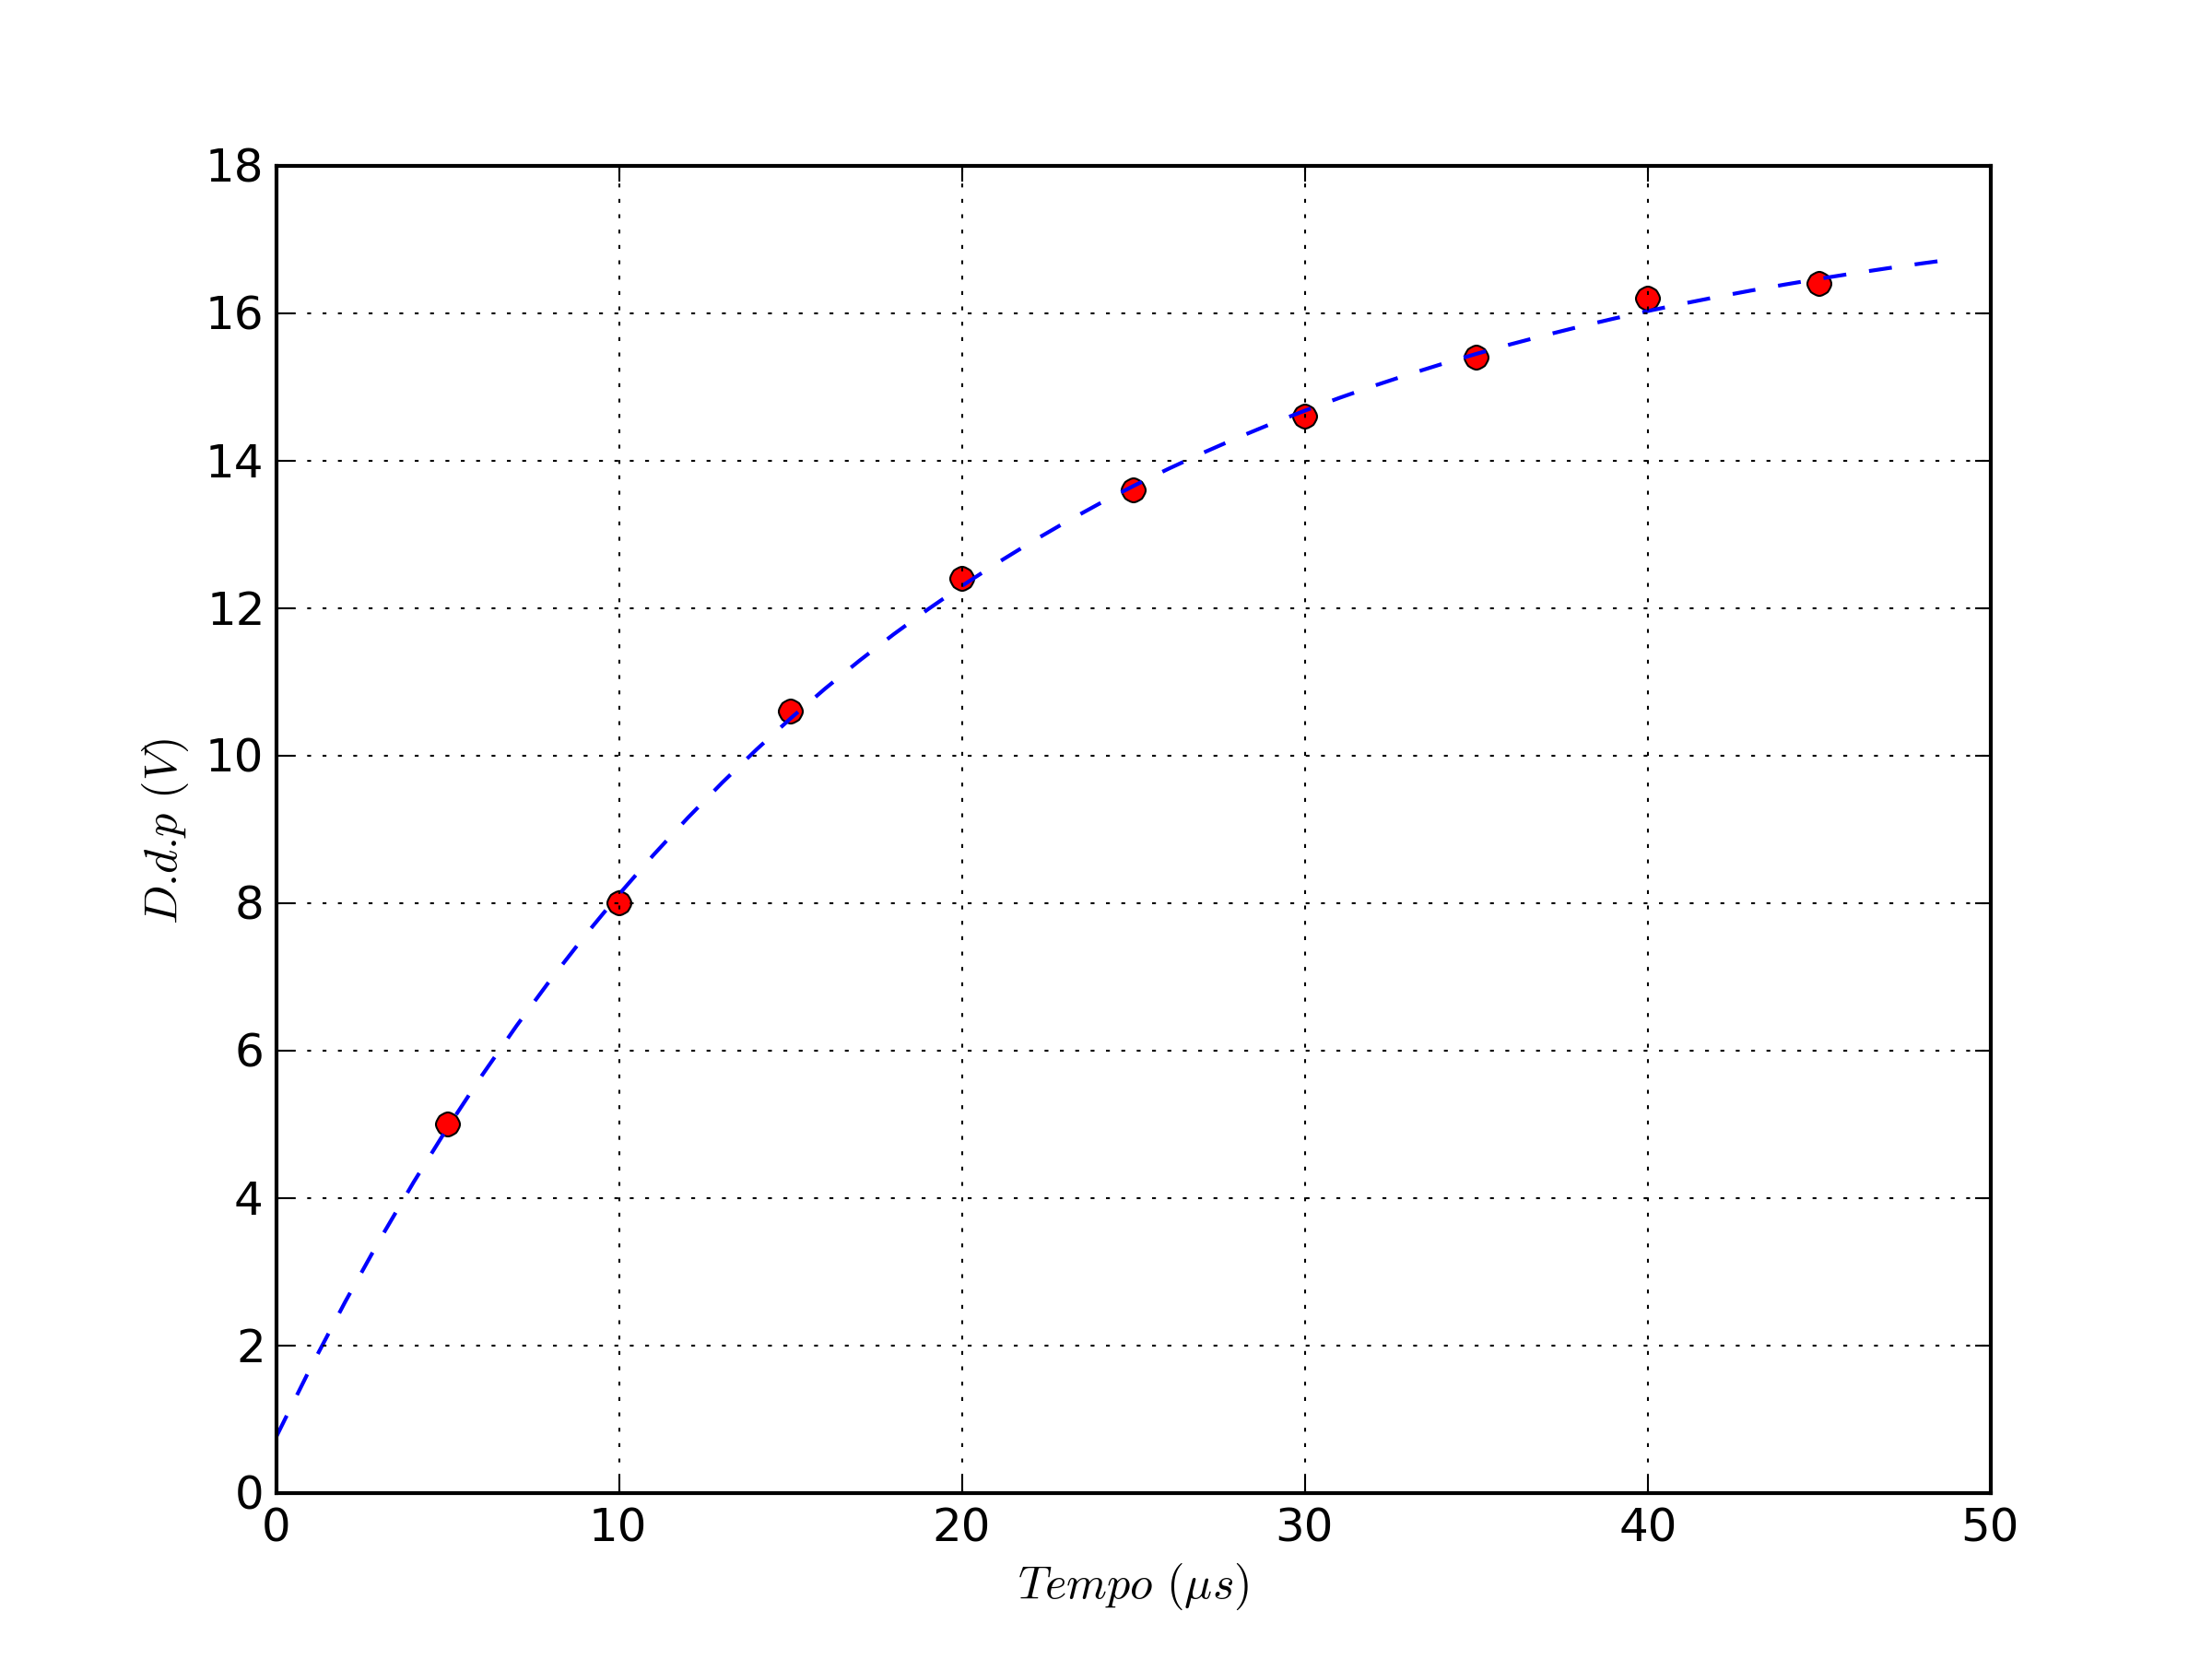
\includegraphics[scale=0.70]{grafici/C3/fitindu.png}
\end{center}

\subsection{Analisi}

\subsubsection{Circuito RC}

Il valore stimato dall'interpolazione è il $\tau=RC$ dell'equazione
$$V_R = V_0 e^{-t/\tau}$$

\subsubsection{Circuito RL}

Il valore stimato dall'interpolazione è il $\tau=L/R$ dell'equazione
$$V_R = V_0 (1-e^{-t/\tau})$$
ove in $R$ abbiamo tenuto conto della resistenza interna dell'induttore, misurata essere 40 Ohm (più err multi).


\subsection{Analisi delle incertezze}


\section{Corrente alternata}
\subsection{Procedimento}

Vogliamo misurare la risposta in frequenza 
\subsection{Raccolta dati}

\subsubsection{Circuito RC}

\begin{center}
 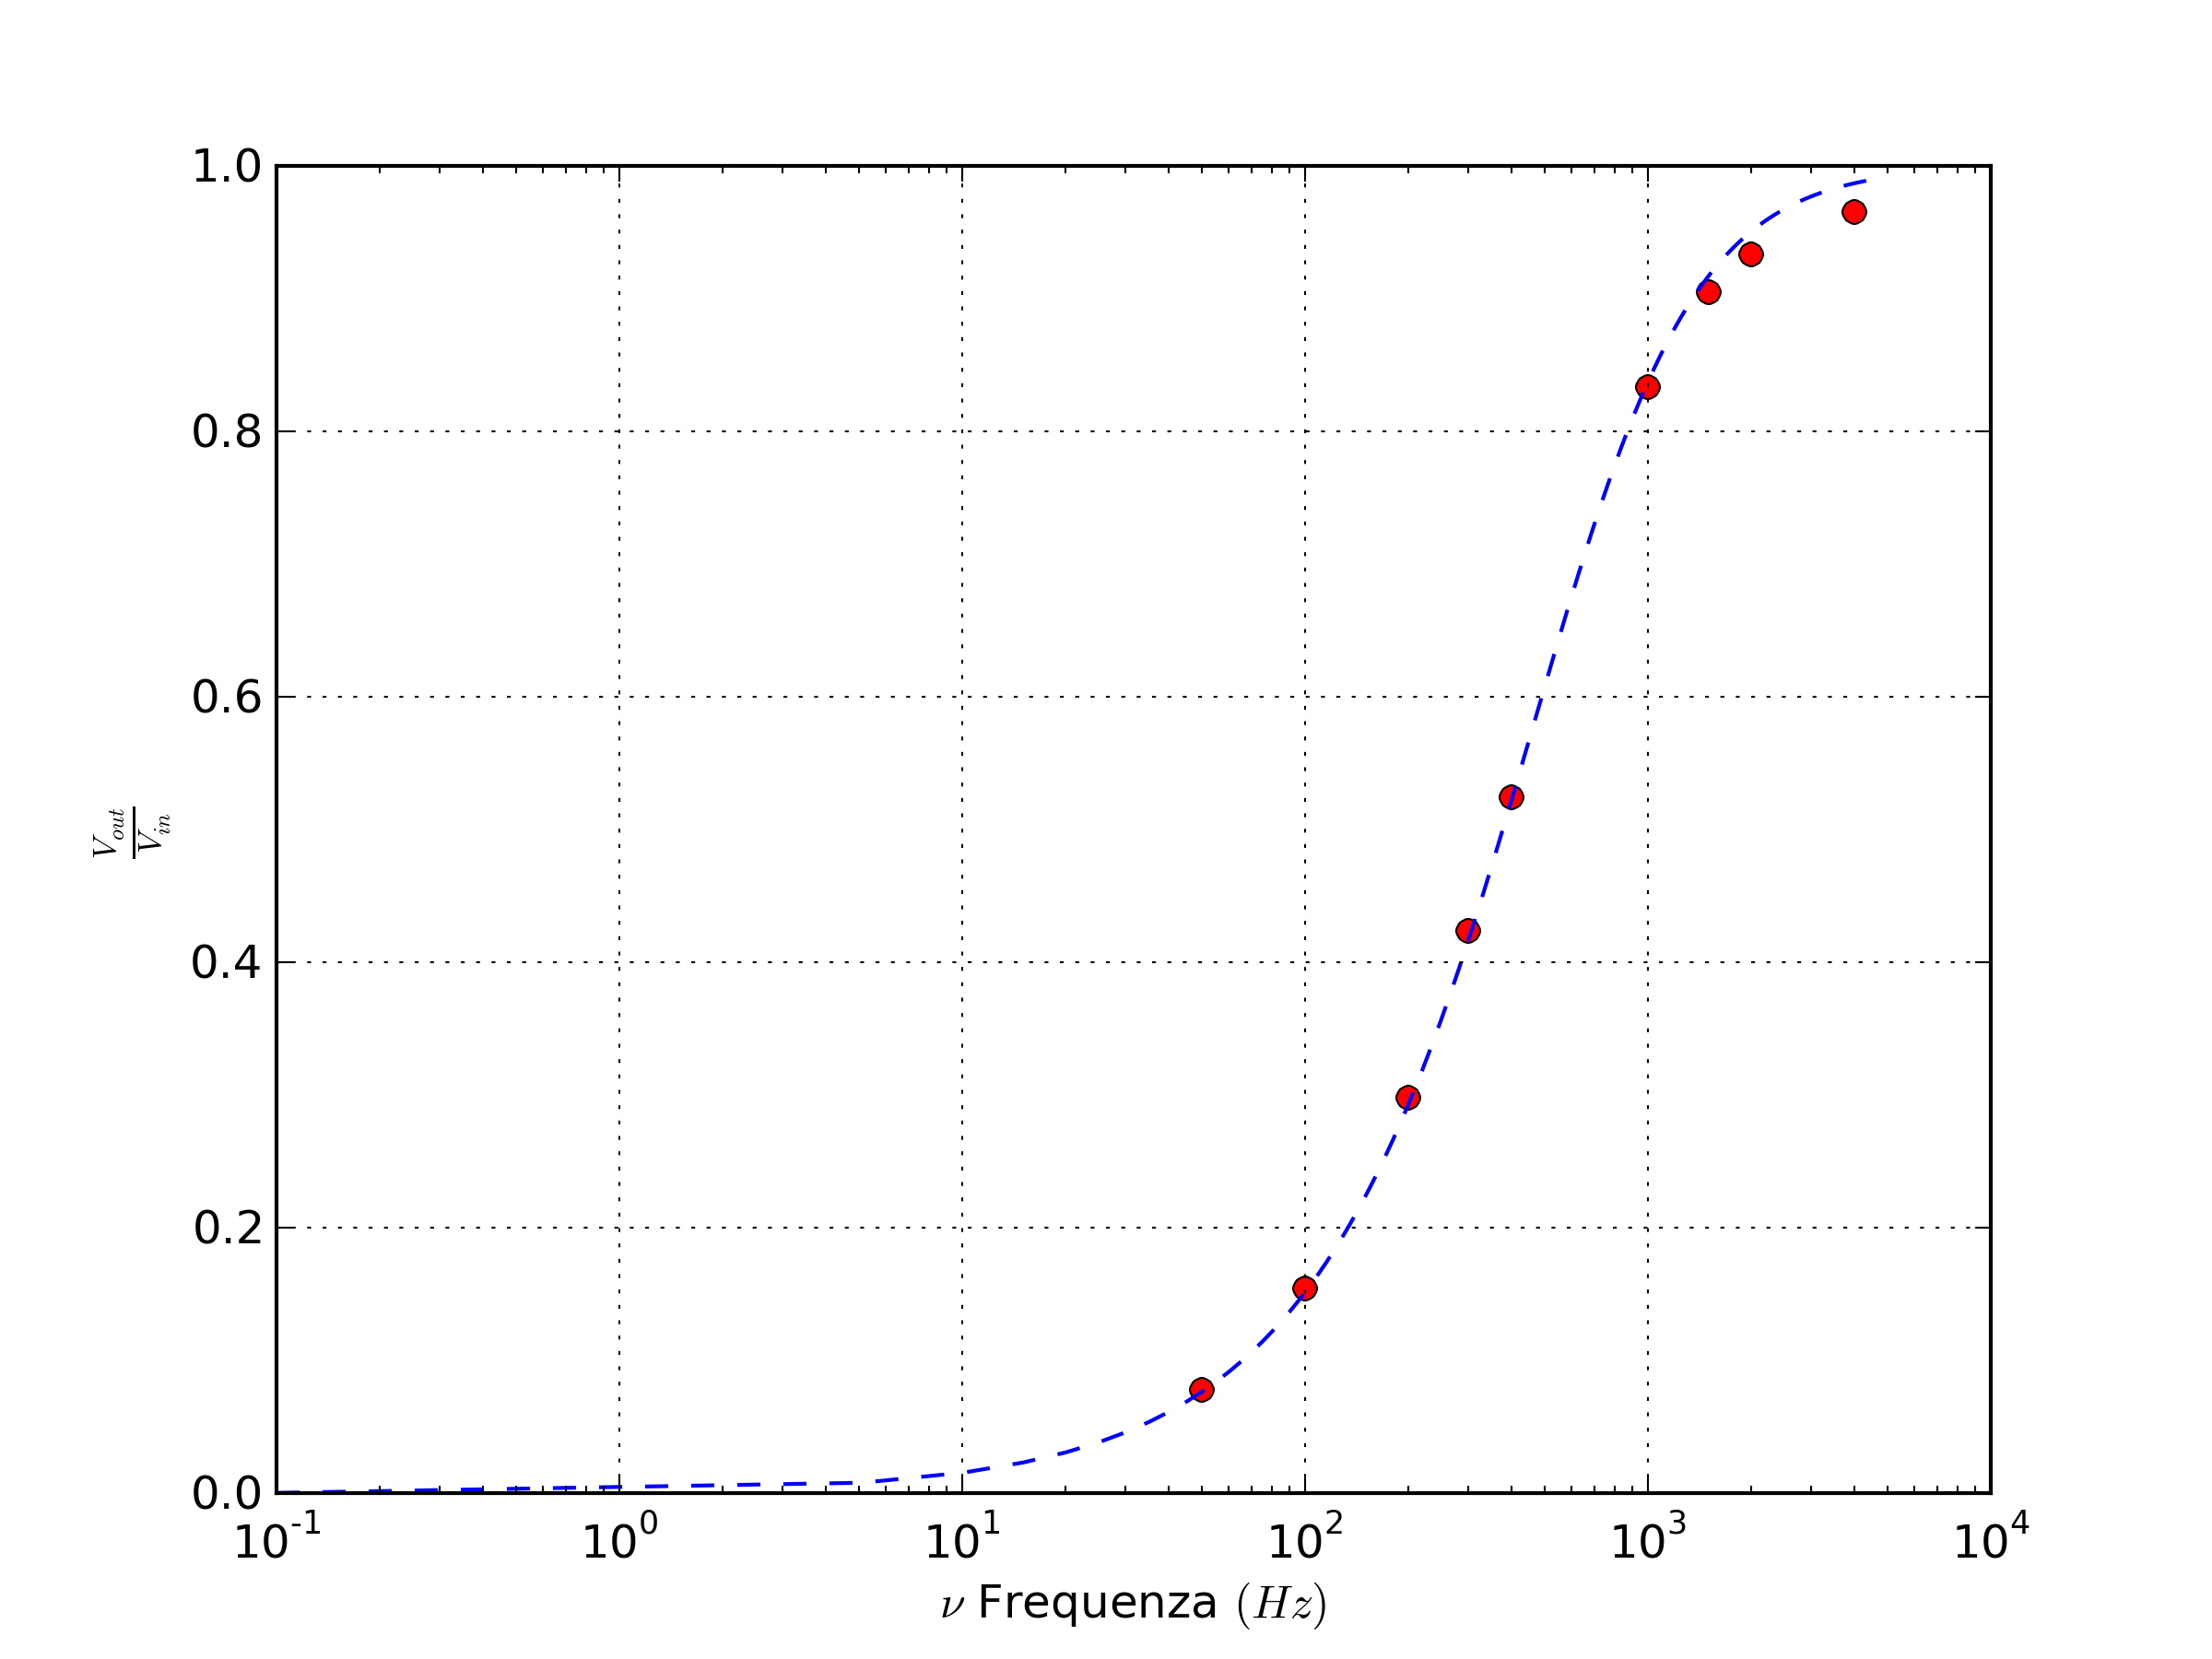
\includegraphics[scale=0.70]{grafici/C3/ddpcond.png}
\end{center}

\begin{center}
\begin{tabular}{*{2}{c}}
Frequenza ($Hz$) & Delta V ($V_{out}/V_{in}$) \\
\midrule
50 & 0.08 \\
100 & 0.15 \\
200 & 0.30 \\
300 & 0.42 \\
400 & 0.52 \\
1000 & 0.83 \\
1500 & 0.90 \\
2000 & 0.93 \\
4000 & 0.97 \\
\end{tabular}
\end{center}


\subsubsection{Circuito RL}

\begin{center}
 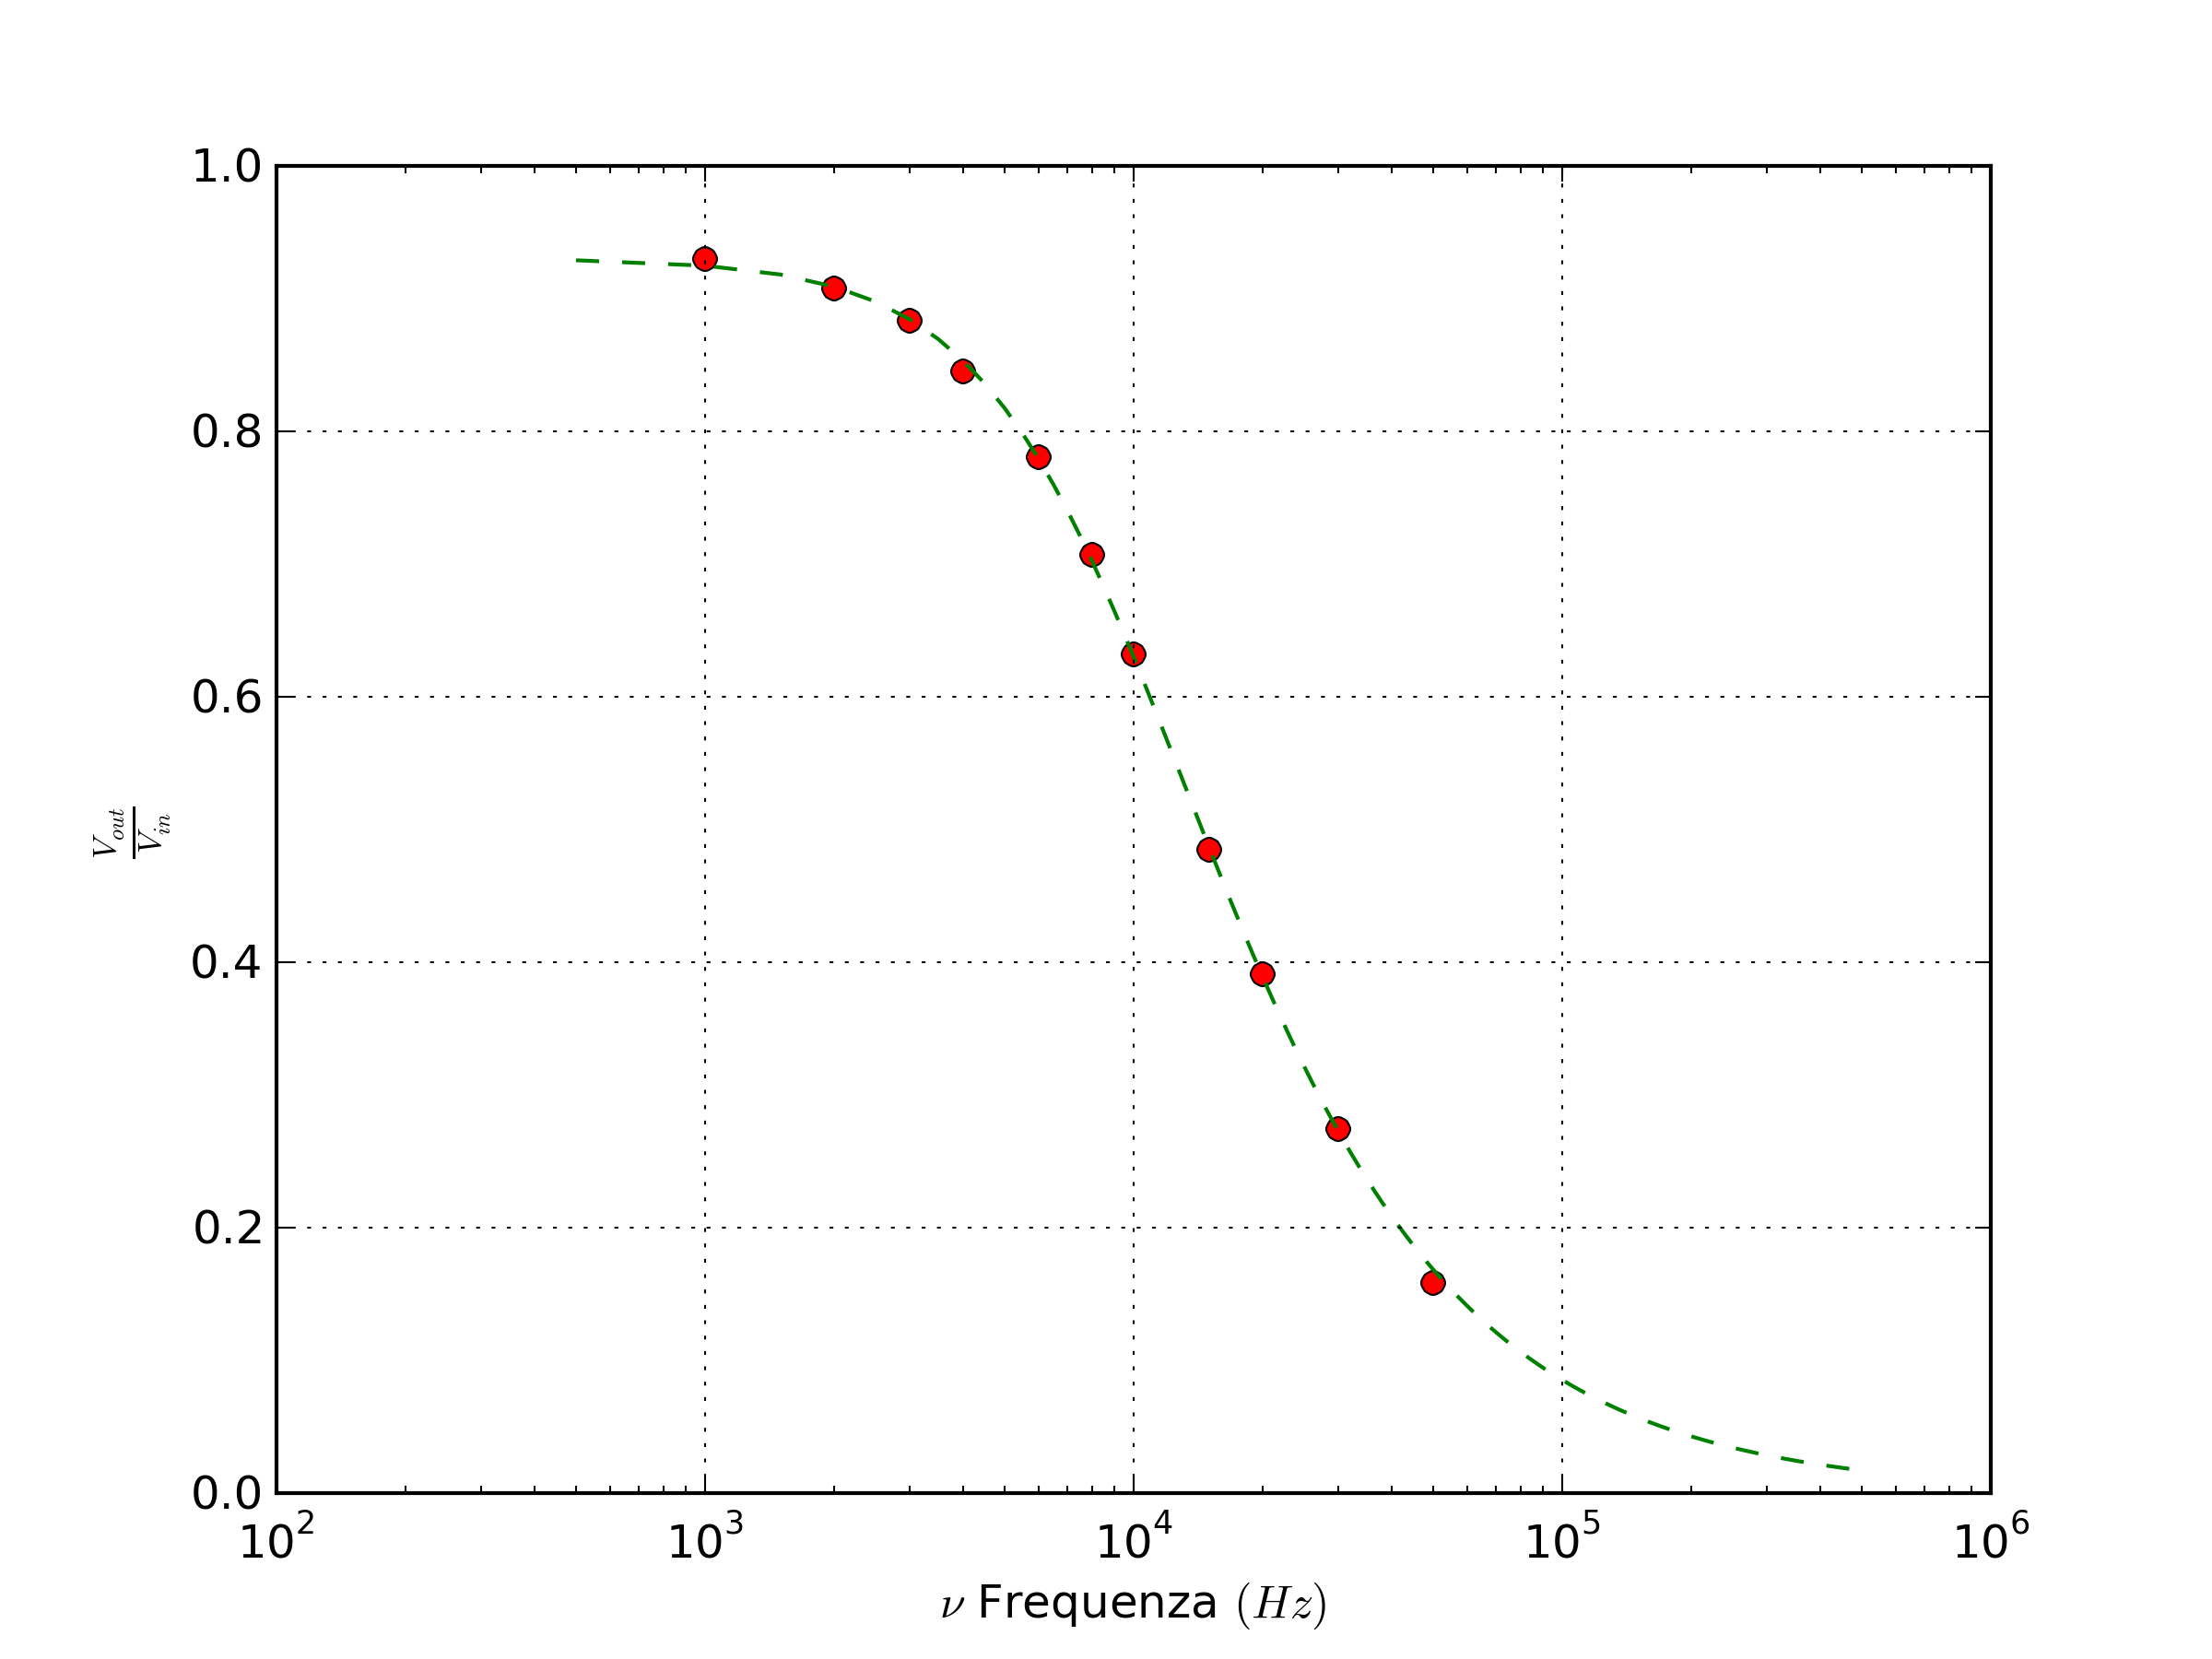
\includegraphics[scale=0.70]{grafici/C3/ddpindu.png}
\end{center}

\begin{center}
\begin{tabular}{*{2}{c}}
Frequenza ($Hz$) & Delta V ($V_{out}/V_{in}$) \\
\midrule
50 & 0.08 \\
100 & 0.15 \\
200 & 0.30 \\
300 & 0.42 \\
400 & 0.52 \\
1000 & 0.83 \\
1500 & 0.90 \\
2000 & 0.93 \\
4000 & 0.97 \\
\end{tabular}
\end{center}

\section{Conclusioni}
\subsubsection{Circuito RC}
\subsubsection{Circuito RL}
